\subsection{Software-Architektur und Design}
\label{sec:software-architektur-und-design}

Dieser Abschnitt überführt die in Abschnitt~4.1 erhobenen funktionalen und nicht-funktionalen Anforderungen sowie die technischen Randbedingungen in einen Architekturentwurf 
für den \textit{CrawlDataTransformer}. Ziel ist es, die wesentlichen strukturellen und organisatorischen Entscheidungen nachvollziehbar herzuleiten und damit die Grundlage 
für die anschließende Implementierung zu schaffen. Im Mittelpunkt stehen dabei die Verantwortlichkeiten der Systembausteine, ihre Beziehungen untereinander sowie die 
Einbindung des Prototyps in die bestehende Systemlandschaft.

Zunächst werden die Architekturziele und Randbedingungen beschrieben und die daraus abgeleiteten Architekturmuster und zentralen Entscheidungen begründet. Anschließend 
wird die Architektur anhand der vier Architektursichten nach Starke (\cite{starke}) dokumentiert. Die Kontextsicht ordnet den \textit{CrawlDataTransformer} in seine 
Systemumgebung ein, während die Bausteinsicht seine statische Zerlegung in fachliche Komponenten, Ports und Adapter beschreibt. Die Laufzeitsicht stellt die Zusammenarbeit 
dieser Bausteine während eines Transformationslaufs dar. Die Verteilungssicht zeigt schließlich ihre Zuordnung zu technischen Ausführungseinheiten sowie die Kommunikation 
mit externen Diensten.

Ergänzend werden sichtübergreifende Architekturkonzepte betrachtet. Dazu gehören das Daten-, Zustands- und Persistenzkonzept, die Gestaltung der externen Schnittstellen, 
die architektonische Unterstützung von Evaluation und Nachvollziehbarkeit sowie die Behandlung von Status- und Fehlerzuständen. Der Abschnitt beschreibt diese Aspekte auf 
Ebene von Verantwortlichkeiten, Beziehungen und grundlegenden Entscheidungen. Die konkrete technische Umsetzung der Komponenten, Datenmodelle und Schnittstellen ist 
Gegenstand von Kapitel~5.

\subsubsection{Architekturziele und Randbedingungen}

Die in Abschnitt~4.1 erhobenen Anforderungen werden im Folgenden zu den für den Architekturentwurf maßgeblichen Architekturzielen verdichtet. Dabei wird zwischen angestrebten 
Qualitätseigenschaften der Architektur und verbindlichen Randbedingungen des Projektkontexts unterschieden. Während die Architekturziele unterschiedliche Lösungsentscheidungen 
zulassen, begrenzen die Randbedingungen den verfügbaren Gestaltungsraum.

\paragraph{Architekturziele:}

Ein primäres Architekturziel ist die Integrationsfähigkeit des \textit{CrawlDataTransformer} bei gleichzeitiger Entkopplung von den bestehenden Nachbarsystemen. 
Die Verarbeitung soll unterschiedliche Eingabekanäle unterstützen und transformierte Produktdaten über eine definierte Schnittstelle an das Zielsystem übergeben können, 
ohne die fachliche Transformationslogik an konkrete Übertragungs- oder Speichertechnologien zu binden.

Eng damit verbunden ist die kontrollierte Verarbeitung gemäß dem vorgegebenen Zielschema. Die Architektur kann die inhaltliche und strukturelle Korrektheit der durch das 
Sprachmodell erzeugten Daten nicht unmittelbar garantieren. Sie muss jedoch ermöglichen, schema-relevante Abweichungen zu erkennen, zu dokumentieren und im weiteren 
Verarbeitungsablauf kontrolliert zu behandeln. Dadurch soll sichergestellt werden, dass nur eindeutig zuordenbare und technisch verarbeitbare Ergebnisse an nachgelagerte 
Schritte übergeben werden.

Ein weiteres primäres Ziel ist die Nachvollziehbarkeit der Transformation. Eingabedaten, Zwischenergebnisse, externe Antworten, Statusübergänge, Bewertungsinformationen 
und Fehlerzustände müssen einem Transformationslauf beziehungsweise einer einzelnen Transformationsanfrage zugeordnet werden können. Diese Rekonstruierbarkeit bildet sowohl 
die Grundlage für die technische Fehleranalyse als auch für die Interpretation unvollständiger oder fehlerhafter Extraktionsergebnisse.

Darauf aufbauend muss die Architektur die wissenschaftliche Evaluation und den Vergleich der Extraktionsansätze unterstützen. Die Ergebnisse der LLM-basierten und der 
regelbasierten Verarbeitung müssen getrennt erhalten bleiben, einer gemeinsamen Referenz zugeordnet und sowohl auf Ebene einzelner Anfragen als auch auf Batch-Ebene 
auswertbar sein. Die konkrete Auswahl und Definition der Bewertungsmetriken erfolgt erst im Evaluationskapitel. Auf Architekturebene ist sicherzustellen, dass die hierfür 
benötigten Ergebnis- und Metadaten verfügbar sind.

Als unterstützendes Ziel soll die Architektur Modularität und Austauschbarkeit fördern. Fachliche Verarbeitungsschritte wie Vorverarbeitung, Extraktion, Validierung, 
Normalisierung, Matching und Evaluation sollen klar voneinander abgegrenzt sein. Ebenso sollen externe Eingabe-, Speicher- und Ausgabesysteme über definierte Schnittstellen 
angebunden werden. Dadurch können einzelne Verarbeitungsschritte, Regeln, Prompts oder externe Dienste angepasst werden, ohne den gesamten Transformationsablauf 
grundlegend verändern zu müssen.

Darüber hinaus muss die Verarbeitung robust gegenüber fachlichen und technischen Fehlern sein. Fehler einer einzelnen Transformationsanfrage sollen nicht zwangsläufig 
zum Abbruch eines gesamten Verarbeitungslaufs führen. Die Architektur soll deshalb eine Fehlerisolation auf Anfrageebene, nachvollziehbare Statusübergänge und die getrennte 
Behandlung interner Verarbeitungsfehler sowie externer Kommunikationsfehler ermöglichen.

Ein weiteres unterstützendes Ziel ist die kontrollierbare und ressourcenbewusste Nutzung des Sprachmodells. Da LLM-Aufrufe variable Laufzeiten und Kosten verursachen, 
müssen Verarbeitung, Tokenverbrauch, Laufzeit und Kosten messbar und steuerbar sein. Zugleich muss die Architektur berücksichtigen, dass Übermittlung und 
Ergebnisbereitstellung durch den externen LLM-Dienst zeitlich getrennt erfolgen können.

\paragraph{Randbedingungen:}

Der Architekturentwurf wird durch mehrere verbindliche Vorgaben des Projektkontexts eingeschränkt. Die Rohdaten werden durch bereits bestehende Crawling-Prozesse 
bereitgestellt. Die Entwicklung oder grundlegende Veränderung des Crawlers ist nicht Bestandteil des Lösungsansatzes. Ebenso ist das Zielschema vorgegeben und wird im 
Rahmen dieser Arbeit nicht erweitert. Der \textit{CrawlDataTransformer} muss sich daher an die vorhandenen Eingabe- und Zielstrukturen anpassen.

Für die LLM-basierte Extraktion und das semantisch unterstützte Produkt-Matching wird ein externer Gemini-Dienst verwendet. Dessen batchbasierte Verarbeitung führt dazu, 
dass die Übermittlung von Anfragen und die spätere Verarbeitung der Antworten nicht als vollständig synchroner Ablauf konzipiert werden können.

Die lokale MongoDB dient ausschließlich als Arbeits-, Transformations- und Evaluationsdatenbank. Sie speichert Eingaben, Zwischenstände, Statusinformationen und 
Bewertungsergebnisse, ersetzt jedoch nicht die produktive Datenhaltung. Die Übergabe transformierter Produktdaten an das Produktivsystem erfolgt ausschließlich über die 
vorgesehene Ziel-API. Ein direkter Schreibzugriff auf die produktive Datenbank ist ausgeschlossen.

Der regelbasierte Vergleichsansatz ist auf das Referenzdatenfeld \textit{ProductSizing} beziehungsweise die Verpackungsgröße begrenzt. Er stellt damit keine vollständige 
Alternative zur LLM-basierten Produktextraktion dar, sondern dient als feldspezifische Baseline für die wissenschaftliche Evaluation. Schließlich ist der 
\textit{CrawlDataTransformer} als Prototyp ausgelegt. Im Vordergrund stehen die konzeptionelle Eignung, die technische Realisierbarkeit und die evaluierbare Gegenüberstellung 
der Ansätze, nicht der vollständige produktive Betrieb.

Aus diesen Architekturzielen und Randbedingungen werden im folgenden Abschnitt die verwendeten Architekturmuster und die zentralen Architekturentscheidungen abgeleitet.


\subsubsection{Architekturmuster und zentrale Architekturentscheidungen}

Die in Abschnitt~4.2.1 beschriebenen Architekturziele und Randbedingungen werden durch eine Kombination mehrerer Architekturmuster und projektspezifischer Entscheidungen 
umgesetzt. Kein einzelnes Muster deckt dabei sämtliche Anforderungen an Integration, fachliche Verarbeitung, zeitlich getrennte LLM-Ausführung und wissenschaftliche Evaluation 
ab. Der \textit{CrawlDataTransformer} verwendet daher eine hybride Architektur aus \textit{Ports and Adapters}, \textit{Pipes and Filters} und einem zentralen 
\textit{TransformationService} zur Orchestrierung. Die Muster erfüllen unterschiedliche Aufgaben und ergänzen sich innerhalb des Gesamtentwurfs.

\paragraph{Entkopplung der Systemgrenzen:}

Die Anbindung technischer Ein- und Ausgabesysteme orientiert sich am Muster \textit{Ports and Adapters}. Ports definieren die vom Anwendungskern benötigten Ein- und 
Ausgangsschnittstellen, während Adapter diese Schnittstellen für konkrete Technologien oder externe Systeme realisieren. Dadurch werden fachliche Komponenten von technischen 
Kommunikations-, Speicher- und Dateiformaten entkoppelt. Eine solche Trennung unterstützt den Austausch und die isolierte Prüfung technischer Integrationen, ohne die fachliche
 Verarbeitung anpassen zu müssen. [Quelle erforderlich]

Diese Entscheidung ist insbesondere relevant, weil der \textit{CrawlDataTransformer} unterschiedliche Arten externer Abhängigkeiten besitzt. Transformationsläufe können über 
verschiedene Eingabekanäle initiiert werden. Für die Extraktion und das Produkt-Matching wird ein externer LLM-Dienst eingebunden, Zwischen- und Zustandsdaten werden lokal 
persistiert und die produktive Übergabe erfolgt über eine separate Ziel-API. Zusätzlich werden Bewertungsergebnisse dateibasiert exportiert. Die fachliche 
Transformationslogik greift nicht unmittelbar auf diese technischen Integrationen zu, sondern verwendet die jeweils dafür vorgesehenen Ports.

Die Trennung der Systemgrenzen ermöglicht außerdem, die lokale Arbeitsdatenhaltung von der produktiven Persistierung abzugrenzen. Der Zugriff auf die lokale Transformations- 
und Produktdatenbank sowie der Export an das Zielsystem werden über unterschiedliche Ausgangsschnittstellen realisiert. Damit kann die lokale Datenbank zur Verwaltung von 
Zwischenständen und Evaluationsergebnissen genutzt werden, ohne einen direkten Schreibzugriff auf die produktive Datenhaltung zu erfordern.

Die zusätzliche Abstraktion durch Ports und Adapter erhöht allerdings die Anzahl der Schnittstellen und erforderlichen Abbildungen zwischen internen und externen 
Datenstrukturen. Dies erzeugt gegenüber einer direkten technischen Kopplung einen höheren strukturellen Aufwand. [Quelle erforderlich] Dieser Aufwand wird in Kauf genommen, 
da Austauschbarkeit, klare Systemgrenzen und die kontrollierte Integration der externen Abhängigkeiten für den Lösungsansatz wesentliche Architekturziele darstellen.

\paragraph{Strukturierung der fachlichen Verarbeitung:}

Die Verarbeitung der Produktdaten orientiert sich am Muster \textit{Pipes and Filters}. Dabei wird eine umfangreiche Transformation in fachlich abgegrenzte 
Verarbeitungsschritte zerlegt. Jeder Filter besitzt eine klar definierte Verantwortung und erzeugt ein Ergebnis, das von nachfolgenden Verarbeitungsschritten weiterverwendet 
werden kann. Diese Zerlegung erleichtert die unabhängige Anpassung einzelner Schritte und ermöglicht, Zwischenergebnisse einem konkreten Verarbeitungsschritt zuzuordnen. 
[Quelle erforderlich]

Für den \textit{CrawlDataTransformer} ist diese Trennung erforderlich, weil die Transformation mehrere Aufgaben mit unterschiedlichen fachlichen Verantwortlichkeiten umfasst. 
Hierzu gehören insbesondere die Vorverarbeitung der HTML-Daten, die Extraktion, die Schema-Validierung, die Normalisierung, das Produkt-Matching, die Evaluation und der Export. 
Änderungen an einer dieser Verantwortlichkeiten sollen nicht zwangsläufig Anpassungen an allen weiteren Verarbeitungsschritten erfordern. Dies betrifft beispielsweise die 
Weiterentwicklung der HTML-Bereinigung, eine Änderung der Extraktionsregeln oder die Ergänzung von Normalisierungsverfahren.

Das Muster wird nicht als eine einzige vollständig synchrone Filterkette umgesetzt. Stattdessen strukturiert es mehrere fachliche Teilpipelines, die zu unterschiedlichen 
Zeitpunkten ausgeführt und durch den \textit{TransformationService} koordiniert werden. Diese Ausgestaltung berücksichtigt, dass die LLM-Verarbeitung zeitlich unterbrochen 
wird und nach der Vorverarbeitung zwei fachlich parallele Extraktionszweige entstehen.

Die Aufteilung in einzelne Filter verbessert die Zuordnung fachlicher Verantwortlichkeiten, führt jedoch zugleich zu zusätzlichen Zwischenzuständen und einem erhöhten 
Koordinationsbedarf. Insbesondere bei verzweigter und zeitlich getrennter Verarbeitung muss nachvollziehbar bleiben, welche Schritte für eine Transformationsanfrage bereits 
abgeschlossen wurden und welche Ergebnisse den folgenden Schritten zur Verfügung stehen.

\paragraph{Mehrphasige und parallele Verarbeitung:}

Eine zentrale Architekturentscheidung ist die Trennung der LLM-basierten Verarbeitung in mehrere zeitlich voneinander unabhängige Phasen. Die Transformationsanfragen werden 
zunächst vorbereitet und gesammelt an den externen LLM-Dienst übermittelt. Die erzeugten Antworten stehen nicht unmittelbar innerhalb desselben synchronen Verarbeitungsvorgangs 
zur Verfügung, sondern werden zu einem späteren Zeitpunkt abgerufen und weiterverarbeitet. Die Architektur muss den Bearbeitungsstand daher zwischen beiden Phasen persistent 
erhalten und die Verarbeitung nach Vorliegen der Ergebnisse fortsetzen können.

Nach der Vorverarbeitung wird zusätzlich ein regelbasierter Extraktionszweig ausgeführt. Beide Zweige verwenden denselben aufbereiteten Produktkontext, unterscheiden sich 
jedoch in ihrem fachlichen Umfang. Der LLM-basierte Zweig erzeugt ein umfassendes strukturiertes Produktergebnis, während der regelbasierte Zweig ausschließlich das 
Referenzdatenfeld \textit{ProductSizing} verarbeitet. Die Zweige stellen daher keine gleichwertigen Alternativen für die gesamte Transformation dar.

Die getrennte Ausführung ist aus der wissenschaftlichen Zielsetzung der Arbeit abgeleitet. Die Ergebnisse beider Ansätze müssen unabhängig voneinander erhalten und 
anschließend für das Referenzdatenfeld mit derselben Ground Truth verglichen werden können. Erst innerhalb der Evaluation werden die relevanten Resultate zusammengeführt. 
Diese Entscheidung ermöglicht den methodisch vorgesehenen Vergleich, erhöht jedoch die Anforderungen an die Zuordnung, Persistenz und Synchronisierung der Ergebnisse.

Aus der mehrphasigen und parallelen Verarbeitung folgt die Entscheidung, Batches und einzelne Transformationsanfragen als getrennte, zustandsbehaftete Arbeitsobjekte zu 
verwalten. Der Batch bildet den übergeordneten Verarbeitungslauf ab, während der Bearbeitungsstand, die Zwischenresultate und mögliche Fehler für jede Transformationsanfrage 
separat nachvollziehbar bleiben. Die konkreten Daten- und Zustandsstrukturen werden in Abschnitt~4.2.6 beschrieben.

\paragraph{Zentrale Orchestrierung:}

Die Koordination der Teilpipelines und Verarbeitungsphasen wird durch den \textit{TransformationService} gebündelt. Dieser stellt keinen weiteren fachlichen Filter dar, 
sondern übernimmt die übergeordnete Orchestrierung des Transformationsablaufs. Zu seinen Aufgaben gehören die Verwaltung von Batches und Transformationsanfragen, der Start 
und die Koordination der Pipelineabschnitte, die Verwaltung der Bearbeitungszustände sowie die Zusammenführung der Ergebnisse für Evaluation und Export.

Die fachliche Logik der einzelnen Verarbeitungsschritte verbleibt in den dafür vorgesehenen Filtern und spezialisierten Komponenten. Der \textit{TransformationService} 
bereinigt, extrahiert, validiert oder normalisiert somit keine Produktdaten selbst. Er koordiniert vielmehr, wann die jeweiligen Verarbeitungsschritte ausgeführt werden und 
welche Ergebnisse für nachfolgende Phasen verfügbar sein müssen. Auch Persistenzzugriffe werden durch ihn beziehungsweise durch die ausgeführten Pipelines koordiniert, während 
die technische Anbindung der Datenbank über entsprechende Ports und Adapter erfolgt.

Die zentrale Orchestrierung verhindert, dass Ablaufsteuerung, Statusverwaltung und Zusammenführung der Extraktionszweige auf mehrere fachliche Filter verteilt werden. 
Gleichzeitig besteht bei einem zentralen Service das Risiko, dass sich dort zu viele fachliche oder technische Verantwortlichkeiten ansammeln. Der Entwurf begrenzt seine 
Rolle deshalb auf die Koordination des Gesamtprozesses. Die eigentliche Verarbeitungslogik sowie die technische Kommunikation mit externen Systemen bleiben in getrennten 
Komponenten gekapselt.

Das Zusammenspiel der Architekturentscheidungen bildet die Grundlage für die nachfolgenden Architektursichten. \textit{Ports and Adapters} strukturiert die Grenzen zu 
Eingabekanälen, Persistenz und externen Diensten. \textit{Pipes and Filters} zerlegt die fachliche Transformation in abgegrenzte Verarbeitungsschritte. Der 
\textit{TransformationService} verbindet diese Strukturen durch die Orchestrierung der parallelen und zeitlich getrennten Teilpipelines. Die daraus entstehenden Bausteine und 
ihre Beziehungen werden im folgenden Abschnitt dargestellt.

\subsubsection{Kontext- und Bausteinsicht}

Die Kontextsicht wurde bereits in Abschnitt~4.1.1 zur Einordnung des \textit{CrawlDataTransformer} in die bestehende Systemlandschaft herangezogen. Sie betrachtet das System 
als Black-Box und zeigt seine Beziehungen zu den vorgelagerten Crawling-Prozessen, dem externen Sprachmodell und dem nachgelagerten Zielsystem. Die Bausteinsicht öffnet diese 
Systemgrenze und stellt die wesentlichen internen Verantwortlichkeiten sowie deren Anbindung an die Systemumgebung dar.

\begin{figure}[H]
    \centering
    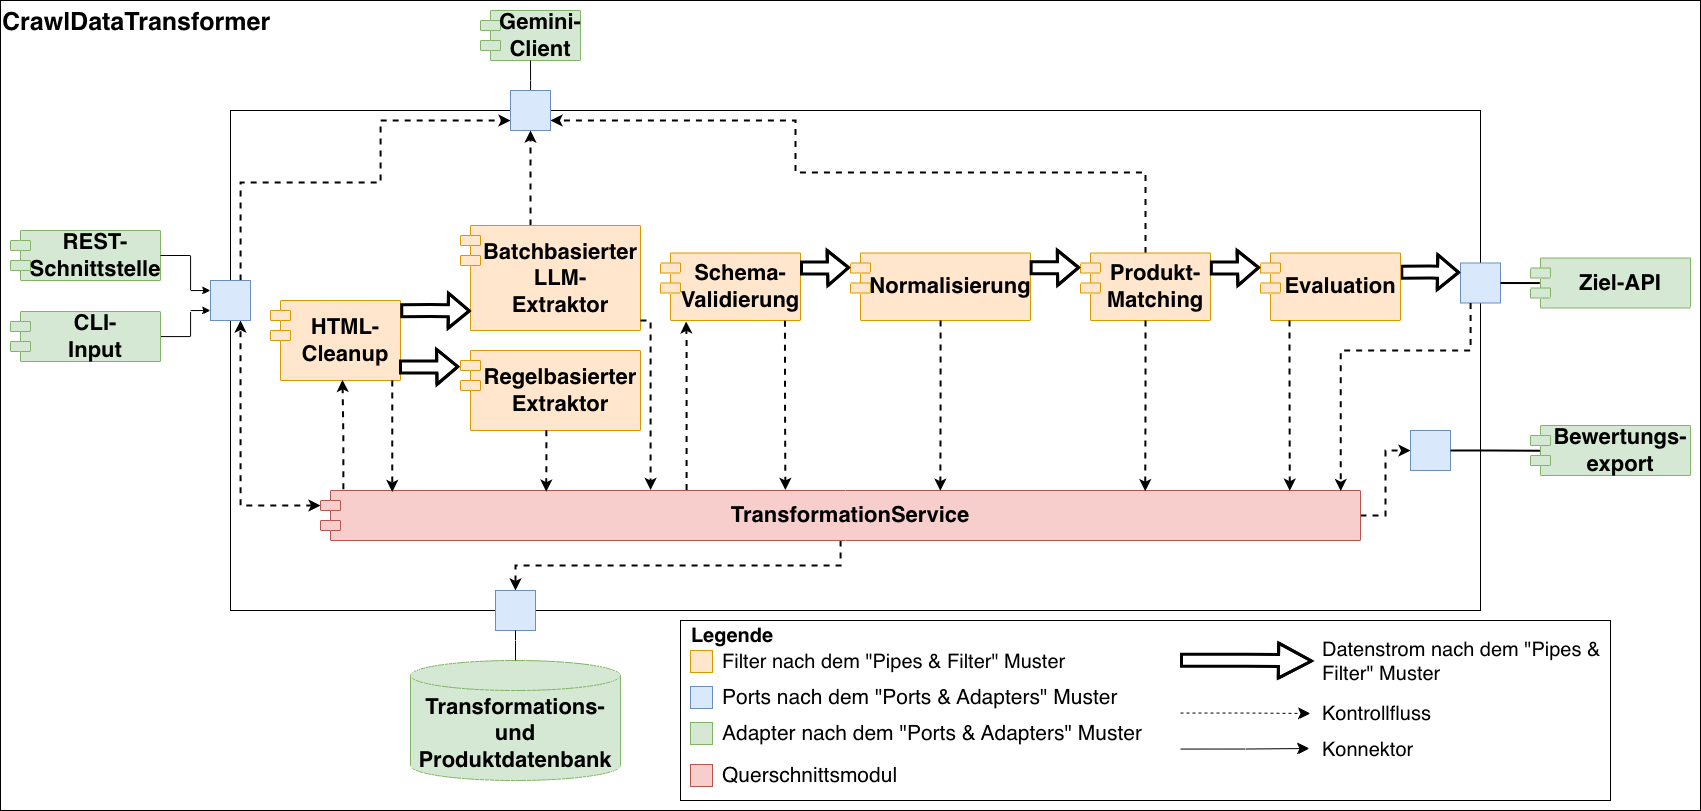
\includegraphics[width=\textwidth]{figures/Bausteinsicht.png}
    \caption{Bausteinsicht des CrawlDataTransformer}
    \label{fig:bausteinsicht}
\end{figure}

Abbildung~\ref{fig:bausteinsicht} zeigt die übergeordnete statische Struktur des \textit{CrawlDataTransformer}. Den fachlichen Kern bilden die Filter der 
Transformationsverarbeitung und der zentrale \textit{TransformationService}. An den Systemgrenzen befinden sich Ports, über die Eingaben, externe LLM-Dienste, Persistenz 
sowie die verschiedenen Exportwege angebunden werden. Die zugehörigen Adapter realisieren die Verbindung zu den konkreten technischen Schnittstellen und externen Ressourcen.

Auf der Eingabeseite können Transformationsläufe über die REST-Schnittstelle oder einen dateibasierten Eingabekanal initiiert werden. Beide Adapter überführen die erhaltenen 
Daten in eine gemeinsame interne Repräsentation und übergeben sie über den Eingangsport an den fachlichen Kern. Nach dieser Überführung können die nachfolgenden 
Verarbeitungsschritte unabhängig vom verwendeten Eingabekanal ausgeführt werden.

Die fachliche Verarbeitung beginnt mit dem HTML-Cleanup. Dieser Baustein bereitet die eingehenden Rohdaten für die Extraktion auf, indem technisch oder gestalterisch bedingte 
Bestandteile reduziert werden und der produktbezogene Informationskontext erhalten bleibt. Das vorverarbeitete HTML bildet anschließend die gemeinsame Grundlage für den 
LLM-basierten und den regelbasierten Extraktionszweig.

Der batchbasierte LLM-Extraktor bereitet die Transformationsanfragen für die externe LLM-Verarbeitung auf und übermittelt sie über den Gemini-Client. Da die Verarbeitung durch 
den LLM-Dienst zeitlich getrennt von der Einreichung erfolgt, werden die Ergebnisse erst zu einem späteren Zeitpunkt abgerufen und der weiteren Verarbeitung zugeführt.

Parallel zur Einreichung der LLM-Anfragen verarbeitet der regelbasierte Extraktor denselben vorverarbeiteten Produktkontext. Seine Verantwortung ist auf das Referenzdatenfeld 
\textit{ProductSizing} beziehungsweise die Verpackungsgröße begrenzt. Der Baustein bildet somit keine vollständige Alternative zur LLM-basierten Produktextraktion, sondern 
erzeugt ein feldspezifisches Ergebnis für die spätere Gegenüberstellung beider Ansätze.

Nach dem Abruf der LLM-Ergebnisse werden diese zunächst durch die Schema-Validierung geprüft. Sie stellt fest, ob die extrahierten Daten strukturell mit dem vorgegebenen 
Schema vereinbar sind. Die anschließende Normalisierung überführt unterschiedliche Darstellungsformen in die für die weitere Verarbeitung vorgesehene Repräsentation. Darauf 
aufbauend gleicht das Produkt-Matching das transformierte Produkt mit vorhandenen Produktdaten ab. Hierfür kann ebenfalls die über den Gemini-Client bereitgestellte 
LLM-Anbindung genutzt werden.

Die Evaluation führt die für das Referenzdatenfeld relevanten Ergebnisse des LLM-basierten und des regelbasierten Zweigs mit den hinterlegten Referenzdaten zusammen. Sie 
erzeugt Bewertungsinformationen auf Ebene einer einzelnen Transformationsanfrage, die anschließend für die vergleichende Auswertung aggregiert werden können. Die Evaluation 
ist dabei von der Schema-Validierung und vom Produktexport getrennt. Sie bewertet die Extraktionsergebnisse, entscheidet jedoch nicht über deren Übergabe an das Zielsystem.

Für die ausgehende Verarbeitung bestehen zwei voneinander getrennte Wege. Das transformierte und gematchte Produktobjekt wird über den Produktexport und den zugehörigen 
Ausgangsport an die Ziel-API übergeben. Die produktive Persistierung verbleibt damit beim nachgelagerten System. Unabhängig davon stellt der Bewertungsexport die erzeugten 
Einzel- und Batchbewertungsergebnisse dateibasiert für die wissenschaftliche Auswertung bereit.

Die lokale Transformations- und Produktdatenbank dient als Arbeits-, Transformations- und Evaluationsdatenbank des Prototyps. In ihr können Eingaben, Verarbeitungszustände, 
Zwischenergebnisse, Produktdaten und Bewertungsinformationen gespeichert werden. Der Zugriff erfolgt über Persistenzschnittstellen, sodass die fachlichen Komponenten nicht 
unmittelbar an die eingesetzte Datenbanktechnologie gebunden sind. Die lokale Datenhaltung ist von der produktiven Persistierung über die Ziel-API zu unterscheiden.

Der \textit{TransformationService} ist in der Bausteinsicht als Querschnittsmodul unterhalb der fachlichen Filter dargestellt. Er koordiniert die Pipelineabschnitte und ihre 
Zustände und führt die Ergebnisse der getrennten Extraktionszweige für die nachgelagerten Verarbeitungsschritte zusammen. Die fachliche Bereinigungs-, Extraktions-, 
Validierungs-, Normalisierungs-, Matching- und Evaluationslogik verbleibt dagegen in den jeweils zuständigen Filtern.

Die Bausteinsicht unterscheidet zwischen Datenstrom, Kontrollfluss und technischer Anbindung. Die breiten Pfeile kennzeichnen die logischen Datenabhängigkeiten der fachlichen 
Verarbeitung nach dem \textit{Pipes-and-Filters}-Muster. Die gestrichelten Pfeile stellen Steuerungs-, Status- und Ergebnisbeziehungen zwischen dem 
\textit{TransformationService}, den Filtern und den Ports dar. Die dünnen durchgezogenen Verbindungen kennzeichnen die technische Anbindung der Ports an die zugehörigen 
Adapter und externen Ressourcen. Die Abbildung beschreibt damit die statische Zerlegung des Systems. Die zeitliche Zusammenarbeit der Bausteine, insbesondere die parallele 
Extraktion und die Unterbrechung durch die asynchrone LLM-Verarbeitung, wird in der folgenden Laufzeitsicht dargestellt.

\subsubsection{Laufzeitsicht der Transformationsverarbeitung}

Die Laufzeitsicht ergänzt die statische Bausteinsicht um die zeitliche Zusammenarbeit der beteiligten Komponenten. Betrachtet wird ein regulärer Transformationslauf auf 
Batch-Ebene. Aufgrund der asynchronen LLM-Verarbeitung besteht dieser nicht aus einer durchgängigen synchronen Verarbeitungskette, sondern aus zwei zeitlich getrennten Phasen.
 Zunächst werden der Batch initialisiert, die Eingabedaten vorverarbeitet und die beiden Extraktionszweige angestoßen. In einer späteren Phase werden die LLM-Ergebnisse 
 abgerufen und durch die nachgelagerten Verarbeitungsschritte geführt.

Die dargestellten Teilnehmer abstrahieren teilweise mehrere technische Komponenten. Die Eingabe fasst den aufrufenden Akteur und den jeweils verwendeten Eingabeadapter 
zusammen. Die lokale Datenbank steht für die Persistenz der Transformations-, Produkt- und Evaluationsdaten. Entsprechend umfasst die Gemini-Anbindung sowohl die interne 
Schnittstelle als auch den externen LLM-Dienst. Der Produkt- und der Bewertungsexport schließen jeweils die zugehörigen Ausgangsschnittstellen und Adapter ein. Die Diagramme 
zeigen damit die logische Interaktion der Architekturbausteine und nicht die konkrete Folge einzelner Methodenaufrufe.

\begin{figure}[H]
    \centering
    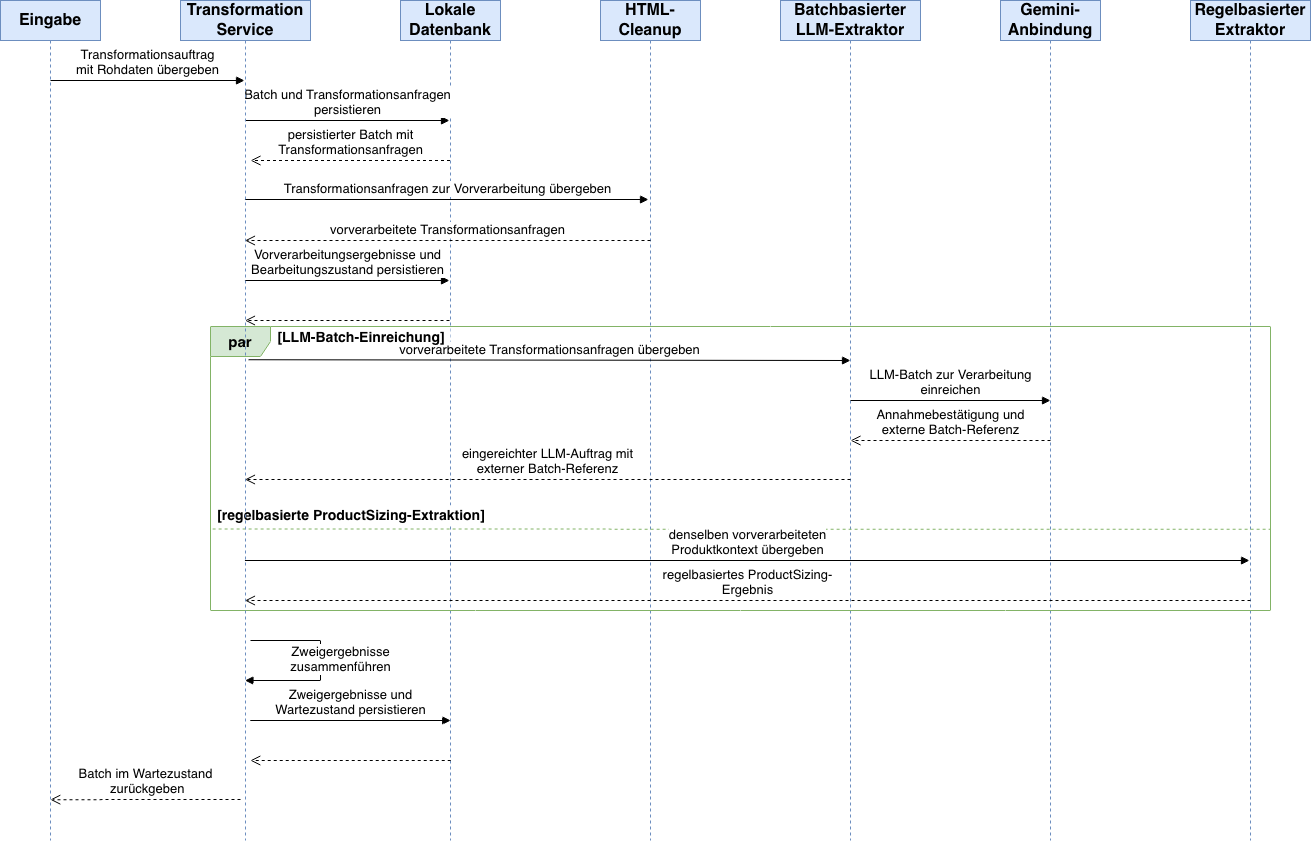
\includegraphics[width=\textwidth]{figures/Laufzeit_Batcherstellung.png}
    \caption{Laufzeitsicht der Batchinitialisierung und Einreichung der Extraktion}
    \label{fig:runtime-batch-creation}
\end{figure}

Abbildung~\ref{fig:runtime-batch-creation} zeigt die erste Phase des Transformationslaufs. Nach der Übergabe eines Transformationsauftrags erzeugt der 
\textit{TransformationService} einen Batch und die darin enthaltenen Transformationsanfragen. Diese Arbeitsobjekte werden in der lokalen Datenbank persistiert, bevor die 
Rohdaten an das HTML-Cleanup übergeben werden. Die Vorverarbeitung reduziert technisch oder gestalterisch bedingte Bestandteile der Eingabe und erzeugt einen gemeinsamen 
Produktkontext für die nachfolgenden Extraktionszweige. Die Vorverarbeitungsergebnisse und der zugehörige Bearbeitungszustand werden anschließend gespeichert.

Auf Grundlage des vorverarbeiteten Produktkontexts werden der LLM-basierte und der regelbasierte Extraktionszweig parallel angestoßen. Der batchbasierte LLM-Extraktor bereitet 
die Anfragen für die externe Verarbeitung vor und reicht sie über die Gemini-Anbindung ein. Als unmittelbares Ergebnis erhält das System lediglich eine externe Batchreferenz. 
Ein fachliches LLM-Extraktionsergebnis liegt zu diesem Zeitpunkt noch nicht vor.

Der regelbasierte Extraktor verarbeitet denselben vorverarbeiteten Produktkontext, liefert jedoch bereits innerhalb dieser Phase ein Ergebnis für das Referenzdatenfeld 
\textit{ProductSizing}. Nach Abschluss beider Zweige ordnet der \textit{TransformationService} die externe LLM-Batchreferenz und das regelbasierte Ergebnis den jeweiligen 
Transformationsanfragen zu. Beide Informationen sowie der Wartezustand werden persistiert. Anschließend wird der Batch an die Eingabeseite zurückgegeben, während die 
Verarbeitung durch den externen LLM-Dienst unabhängig davon fortgesetzt wird.

\begin{figure}[H]
    \centering
    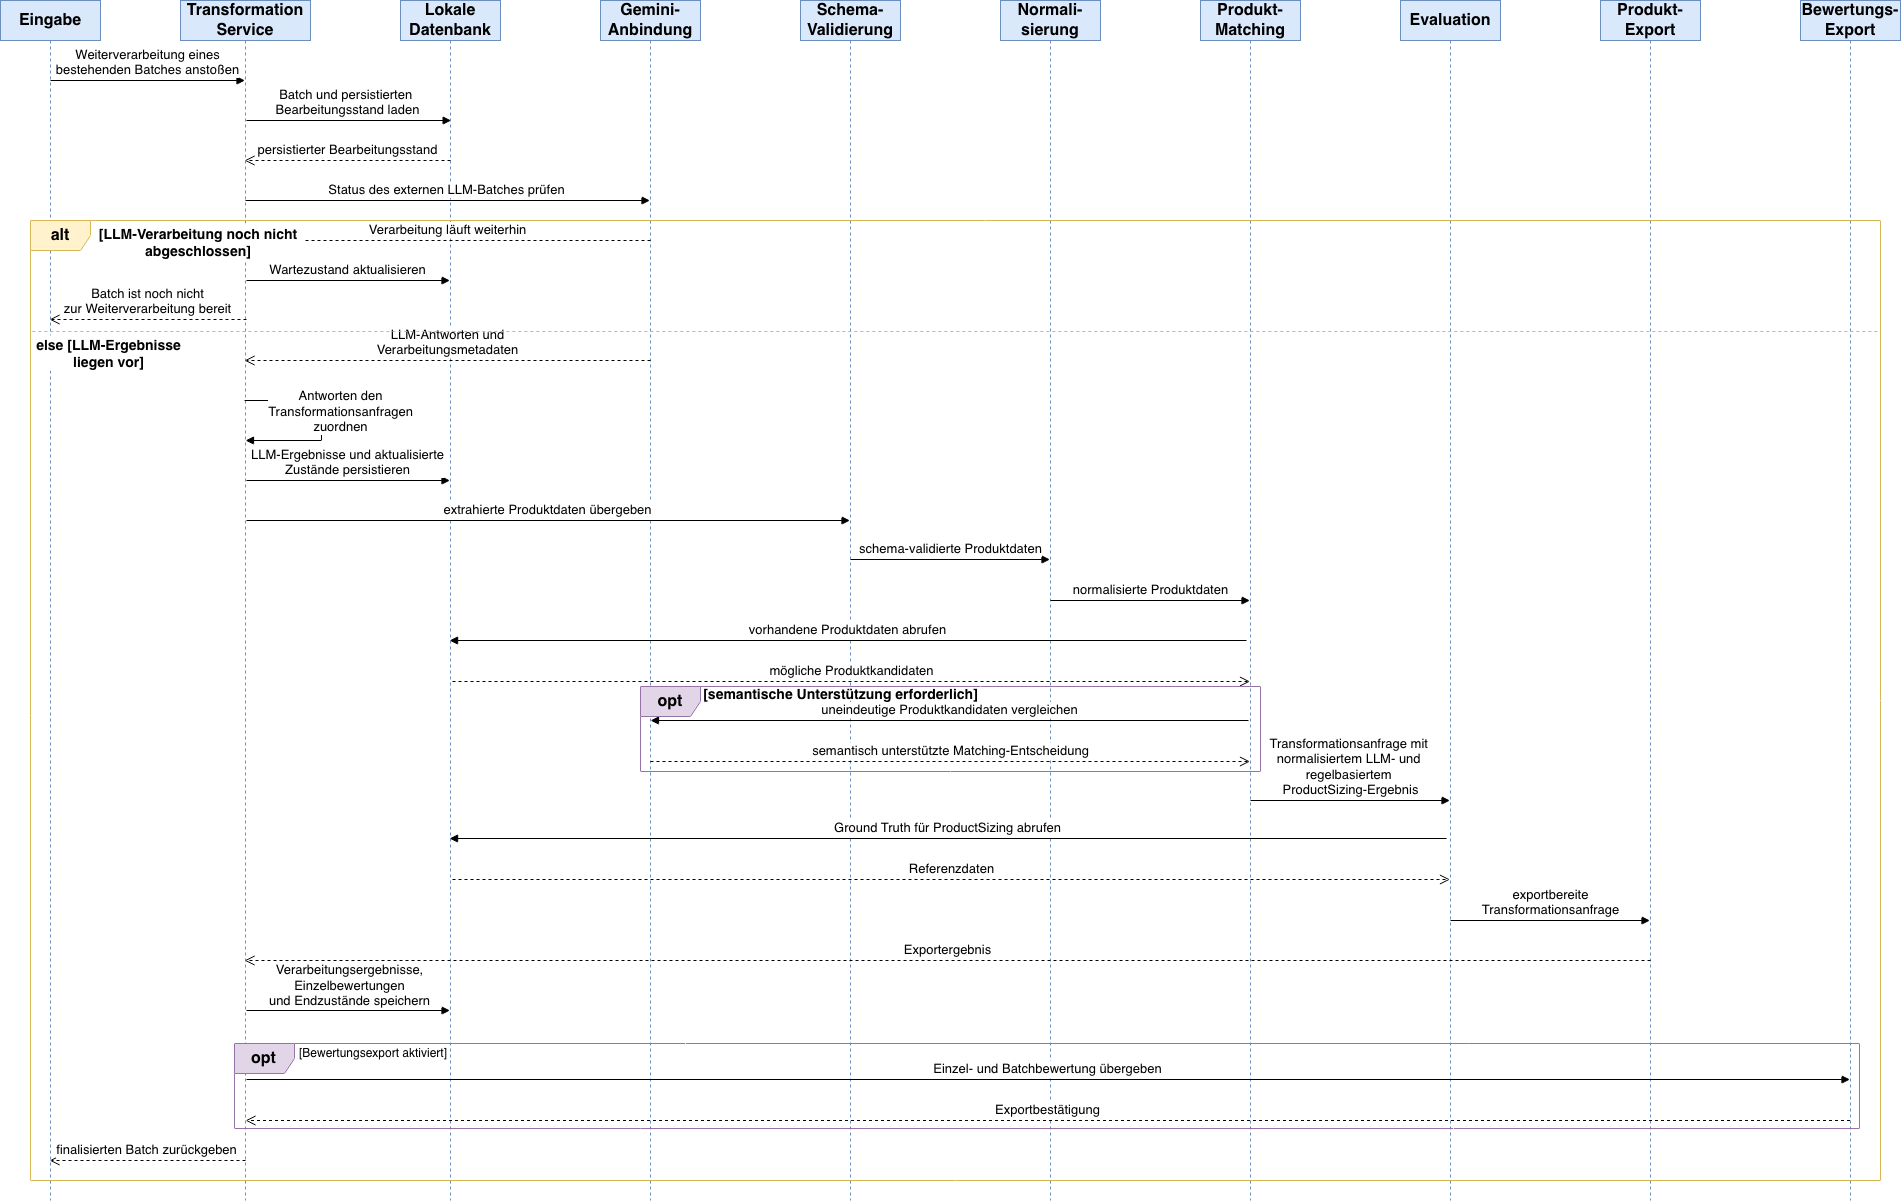
\includegraphics[width=\textwidth]{figures/Laufzeit_Extraktion.png}
    \caption{Laufzeitsicht der LLM-Ergebnisverarbeitung und nachgelagerten Transformation}
    \label{fig:runtime-extraction}
\end{figure}

Abbildung~\ref{fig:runtime-extraction} stellt die zweite Phase dar. Sie wird durch einen separaten Aufruf für einen bereits bestehenden Batch angestoßen. Der 
\textit{TransformationService} lädt den persistierten Bearbeitungsstand und fragt über die Gemini-Anbindung den Status des externen LLM-Batches ab. Ist die externe 
Verarbeitung noch nicht abgeschlossen, wird der Wartezustand beibehalten und der Eingabeseite mitgeteilt, dass der Batch noch nicht weiterverarbeitet werden kann. 
Detaillierte Fehlerfälle der externen Verarbeitung werden in Abschnitt~4.2.9 betrachtet.

Liegen die LLM-Ergebnisse vor, werden die Antworten den ursprünglichen Transformationsanfragen zugeordnet und gemeinsam mit den aktualisierten Zuständen persistiert. 
Anschließend beginnt die nachgelagerte fachliche Verarbeitung. Die Schema-Validierung prüft zunächst die strukturelle Vereinbarkeit der extrahierten Daten mit dem 
vorgegebenen Schema. Nur entsprechend verarbeitbare Ergebnisse werden an die Normalisierung weitergegeben, die unterschiedliche Darstellungsformen in die vorgesehene 
interne Repräsentation überführt.

Das Produkt-Matching gleicht die normalisierten Produktdaten mit den lokal verfügbaren Produktdaten ab. Sind die ermittelten Kandidaten nicht eindeutig, kann die 
Gemini-Anbindung ergänzend für eine semantisch unterstützte Matching-Entscheidung verwendet werden. Das daraus hervorgehende Matching-Ergebnis bleibt gemeinsam mit den 
übrigen Zwischenständen Bestandteil der jeweiligen Transformationsanfrage.

Die Evaluation vergleicht das normalisierte LLM-Ergebnis und das bereits gespeicherte regelbasierte \textit{ProductSizing}-Ergebnis mit der zugehörigen Ground Truth. Sie 
erzeugt daraus Bewertungsinformationen für die einzelne Transformationsanfrage. Diese Bewertung ist vom Produktexport getrennt und entscheidet nicht über dessen Freigabe. 
Insbesondere werden die Evaluationsergebnisse nicht als Bestandteil des Produktobjekts an das Zielsystem übergeben.

Der Produktexport überführt das gematchte Produkt in die für die Ziel-API erforderliche Darstellung und übermittelt es an das nachgelagerte System. Verarbeitungsergebnisse, 
Einzelbewertungen und Endzustände werden während der Verarbeitung lokal persistiert. Nach Abschluss der Transformationsanfragen bildet der \textit{TransformationService} 
eine Batchzusammenfassung und aggregiert die vorhandenen Einzelbewertungen. Sofern der Bewertungsexport aktiviert ist, werden die Einzel- und Batchbewertungsergebnisse 
zusätzlich in dateibasierter Form für die wissenschaftliche Auswertung bereitgestellt.

Die beiden Laufzeitdiagramme verdeutlichen damit insbesondere die Trennung zwischen Einreichung und Verarbeitung der LLM-Ergebnisse. Gleichzeitig zeigen sie, wie persistierte 
Zwischenzustände die zeitlich unterbrochene Verarbeitung ermöglichen und wie der LLM-basierte sowie der regelbasierte Extraktionszweig innerhalb der Evaluation wieder 
zusammengeführt werden.

\subsubsection{Verteilungssicht}

Die Verteilungssicht nach Starke (\cite{starke}) ordnet die Softwarebausteine den technischen Ausführungseinheiten zu und stellt deren Kommunikationsbeziehungen dar. 
Abbildung~\ref{fig:deployment-view} zeigt das prototypische, containerbasierte Betriebsmodell des \textit{CrawlDataTransformer}. Im Mittelpunkt steht die über die 
REST-Schnittstelle nutzbare Ausführung. Die Abbildung beschreibt keine produktive Zielinfrastruktur, sondern die für Entwicklung, Erprobung und Evaluation vorgesehene
 Laufzeitumgebung.

\begin{figure}[H]
    \centering
    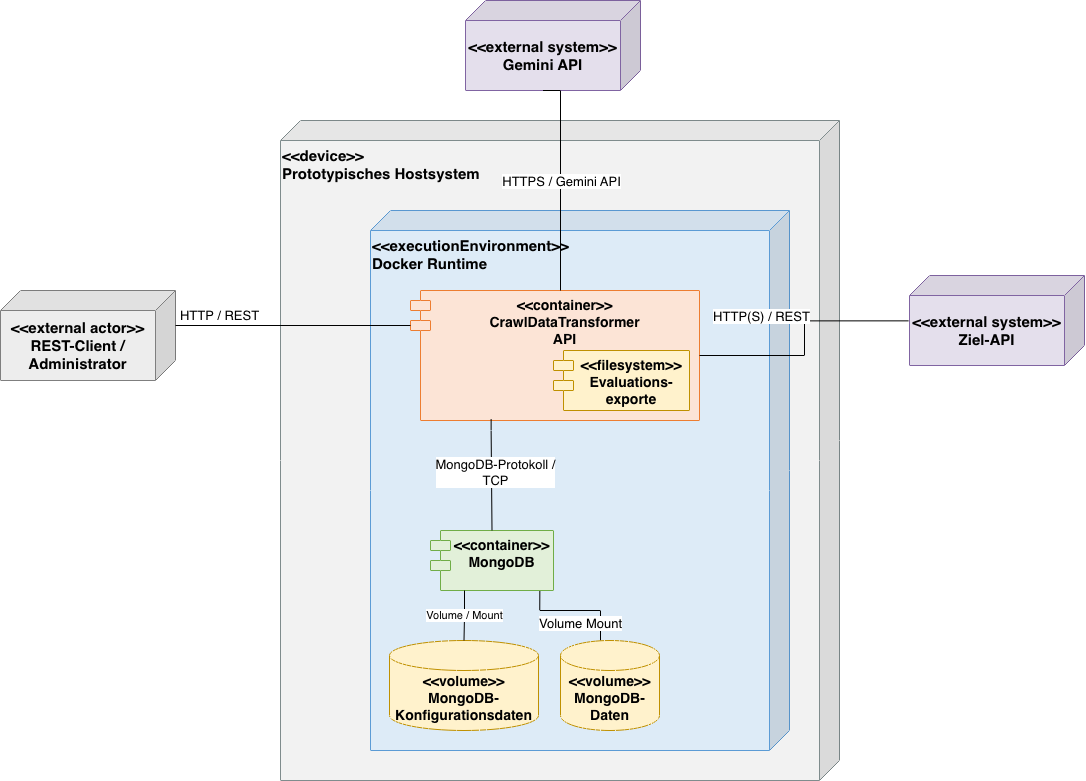
\includegraphics[width=\textwidth]{figures/Verteilungssicht.png}
    \caption{Verteilungssicht des CrawlDataTransformer im prototypischen Betriebsumfeld}
    \label{fig:deployment-view}
\end{figure}

Innerhalb des prototypischen Hostsystems stellt eine Docker-Laufzeitumgebung die benötigten Ausführungseinheiten bereit. Der \textit{CrawlDataTransformer} und die lokale 
MongoDB werden in getrennten Containern betrieben. Der Anwendungscontainer umfasst die REST-Schnittstelle, den fachlichen Anwendungskern sowie die für die Verarbeitung 
benötigten Adapter. Externe Aufrufer greifen über HTTP und REST auf die veröffentlichte Schnittstelle des Containers zu. Die Kommunikation zwischen dem Anwendungs- und dem 
Datenbankcontainer erfolgt über das MongoDB-Protokoll innerhalb des gemeinsamen Docker-Netzwerks.

Die Trennung der Anwendung von der Datenbank ermöglicht, beide Ausführungseinheiten unabhängig voneinander bereitzustellen und zu verwalten. Der MongoDB-Container bindet 
jeweils ein Volume für die Datenbestände und die internen Konfigurationsdaten ein. Dadurch ist die lokale Persistenz vom Lebenszyklus eines einzelnen Datenbankcontainers 
getrennt. Die MongoDB übernimmt ausschließlich die Funktion einer Arbeits-, Transformations- und Evaluationsdatenbank. Sie speichert unter anderem Transformationsanfragen, 
Bearbeitungszustände, Zwischenresultate, Produktdaten und Bewertungsinformationen. Eine direkte Verbindung zur produktiven Datenbank des Zielsystems besteht nicht.

Der dateibasierte Bewertungsexport wird innerhalb des Anwendungscontainers abgelegt. Er stellt die zuvor erzeugten Einzel- und Batchbewertungen für die wissenschaftliche 
Auswertung bereit. Im dargestellten prototypischen Betriebsmodell ist für dieses Verzeichnis kein eigenständiges Volume vorgesehen. Die Exportdateien sind daher an den 
Lebenszyklus des Anwendungscontainers gebunden und besitzen nicht dieselbe dauerhafte Persistenz wie die in MongoDB gespeicherten Daten. Diese Einschränkung ist für das 
lokale Evaluationsszenario akzeptiert, müsste für einen dauerhaften Betrieb jedoch durch einen persistenten Speicher ergänzt werden.

Außerhalb der lokalen Laufzeitumgebung befinden sich die Gemini API und die Ziel-API als eigenständige Nachbarsysteme. Der Anwendungscontainer kommuniziert über HTTPS mit 
der Gemini API. Diese Verbindung wird sowohl für die batchbasierte LLM-Verarbeitung als auch für die optionale semantische Unterstützung des Produkt-Matchings verwendet. 
Die Ziel-API wird über eine REST-basierte HTTP(S)-Verbindung angesprochen und übernimmt die abschließende Validierung und produktive Persistierung der exportierten 
Produktdaten. Der konkrete physische Betriebsort der Ziel-API ist für den Architekturentwurf des Prototyps nicht festgelegt. Maßgeblich ist ihre Einbindung als technisch 
und organisatorisch getrenntes Nachbarsystem.

Die zeitlich getrennte LLM-Verarbeitung erfordert im prototypischen Verteilungsmodell keine zusätzliche lokale Ausführungseinheit. Sowohl die Einreichung der LLM-Batches 
als auch der spätere Abruf und die Weiterverarbeitung der Ergebnisse erfolgen innerhalb desselben Anwendungscontainers. Die für diese Unterbrechung benötigten Zustände und 
externen Batchreferenzen werden in der lokalen MongoDB persistiert. Ein separater Worker, eine lokale Nachrichtenwarteschlange oder ein Callback-Endpunkt für automatische 
Rückmeldungen des LLM-Dienstes sind nicht Bestandteil des aktuellen Entwurfs.

Neben der dargestellten REST-Ausführung kann der Anwendungskern über die Kommandozeilenschnittstelle lokal gestartet werden. In diesem Fall werden Eingabedateien aus dem 
Dateisystem des Hostsystems geladen, während für Persistenz und externe Kommunikation dieselben technischen Schnittstellen verwendet werden. Da diese Ausführungsform keine 
abweichende fachliche Architektur darstellt, wird sie im Verteilungsdiagramm nicht als zusätzlicher Knoten modelliert. Ebenso bleiben reine Entwicklungs- und 
Administrationswerkzeuge zugunsten der Übersicht unberücksichtigt.

Das dargestellte Verteilungsmodell ist auf den prototypischen Betrieb ausgerichtet. Maßnahmen für horizontale Skalierung, Hochverfügbarkeit, Lastverteilung oder den Betrieb 
mehrerer Anwendungsinstanzen sind nicht vorgesehen. Die Verteilungssicht zeigt damit die technischen Rahmenbedingungen, unter denen die zuvor beschriebene 
Transformationsverarbeitung ausgeführt wird. Die dabei persistent verwalteten Arbeitsobjekte, Beziehungen und Zustände werden im folgenden Abschnitt näher betrachtet.

\subsubsection{Daten-, Zustands- und Persistenzkonzept}

Die mehrphasige und zeitlich unterbrochene Transformationsverarbeitung erfordert, dass Eingaben, Zwischenergebnisse und Bearbeitungszustände über einzelne Pipelineabschnitte 
hinweg erhalten bleiben. Das Daten- und Persistenzkonzept unterscheidet deshalb zwischen übergeordneten Verarbeitungsbatches, einzelnen Transformationsanfragen, lokal 
verwalteten Produktdaten und den für die Evaluation benötigten Referenzdaten. Die konkreten MongoDB-Dokumente, Mapper und Repository-Implementierungen werden erst in 
Kapitel~5 beschrieben. Im Folgenden stehen die fachlichen Arbeitsobjekte, ihre Beziehungen sowie die durch ihre Zustände repräsentierten Verarbeitungsphasen im Vordergrund.

\begin{figure}[H]
    \centering
    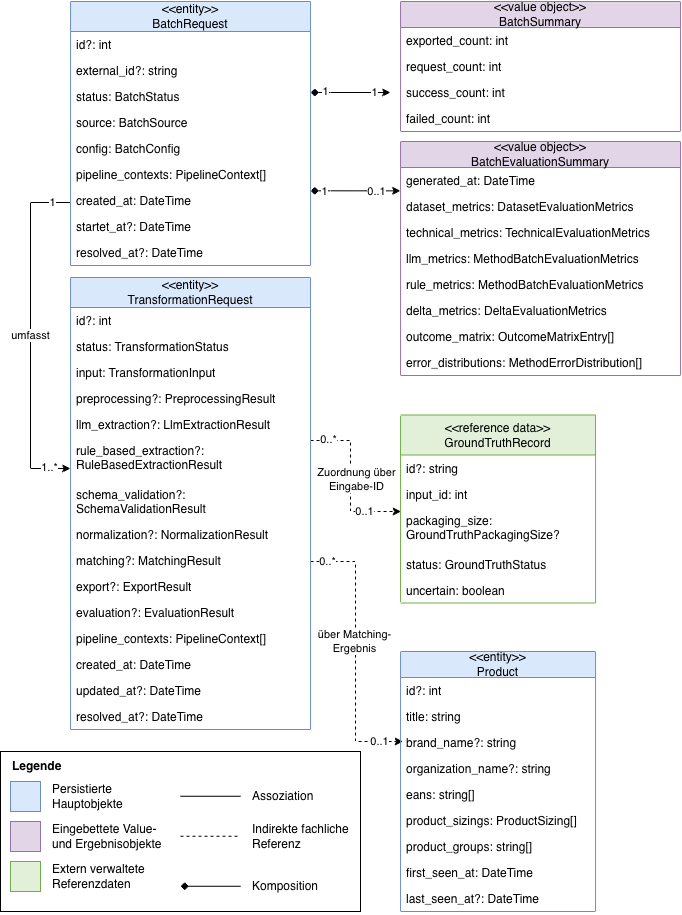
\includegraphics[width=\textwidth]{figures/DB_konzeptionell.png}
    \caption{Konzeptionelles Daten- und Persistenzmodell des CrawlDataTransformer}
    \label{fig:conceptual-data-model}
\end{figure}

\paragraph{Konzeptionelles Datenmodell:}

Abbildung~\ref{fig:conceptual-data-model} zeigt die zentralen persistenten Arbeitsobjekte und ihre fachlichen Beziehungen. Ein \textit{BatchRequest} repräsentiert einen 
zusammengehörigen Transformationslauf und umfasst mindestens einen \textit{TransformationRequest}. Er enthält die Herkunft und Konfiguration des Laufs, die externe Referenz 
der LLM-Batch-Verarbeitung, den aktuellen Bearbeitungszustand sowie die zur Ausführung gehörenden Kontextinformationen. Der \textit{BatchRequest} ist damit kein fachliches 
Produktobjekt, sondern dient der Koordination und Aggregation mehrerer einzelner Transformationen.

Die operative Zusammenfassung eines Batches wird im eingebetteten \textit{BatchSummary} gespeichert. Der \textit{request\_count} gibt die Gesamtzahl der enthaltenen 
Transformationsanfragen an. Der \textit{success\_count} umfasst diejenigen Anfragen, die die verpflichtenden Transformationsschritte bis zur Exportbereitschaft erfolgreich 
abgeschlossen haben und sich im Zustand \textit{READY\_FOR\_EXPORT} oder \textit{EXPORTED} befinden. Davon getrennt weist der \textit{exported\_count} ausschließlich 
erfolgreich an die Ziel-API übergebene Anfragen aus. Der \textit{failed\_count} enthält die Anzahl der fehlgeschlagenen Einzelanfragen. Dadurch bleibt auch bei einem teilweise 
erfolgreichen Batch erkennbar, wie viele Produktdatensätze vollständig verarbeitet, exportiert oder aufgrund eines Fehlers ausgeschlossen wurden.

Die aggregierten Evaluationsinformationen werden in einer separaten \textit{BatchEvaluationSummary} gespeichert. Sie fasst die auf Ebene einzelner Transformationsanfragen 
erzeugten Bewertungen zusammen und trennt unter anderem Datensatz-, technische und methodenspezifische Kennzahlen. Die konkrete Definition und Berechnung dieser Metriken 
erfolgt in Abschnitt~4.2.8 und im Evaluationskapitel. Die Trennung vom operativen \textit{BatchSummary} verhindert, dass der technische Bearbeitungsfortschritt mit der 
wissenschaftlichen Bewertung der Extraktionsansätze vermischt wird.

Der \textit{TransformationRequest} bildet die zentrale Verarbeitungseinheit für einen einzelnen Produktdatensatz. Das lokal persistierte Objekt \textit{Product} dient dem 
Produkt-Matching und der Vorbereitung des Exports. Die Zuordnung erfolgt indirekt über das Matching-Ergebnis einer Transformationsanfrage. Ein lokales Produkt ist dabei nicht 
mit dem produktiven Datensatz des Zielsystems gleichzusetzen. Die produktive Validierung und Speicherung erfolgen weiterhin ausschließlich über die Ziel-API.

Die \textit{GroundTruthRecord}-Objekte werden getrennt von den regulären Arbeitsobjekten als Referenzdatenbasis verwaltet. Die Zuordnung zu einer Transformationsanfrage 
erfolgt über die Kennung der ursprünglichen Eingabe. Eine Ground Truth enthält die erwartete Verpackungsgröße sowie Informationen über den Annotations- und Auswertungszustand. 
Sie wird ausschließlich für die Evaluation herangezogen und stellt kein Ergebnis der Transformationspipeline dar.

\begin{figure}[H]
    \centering
    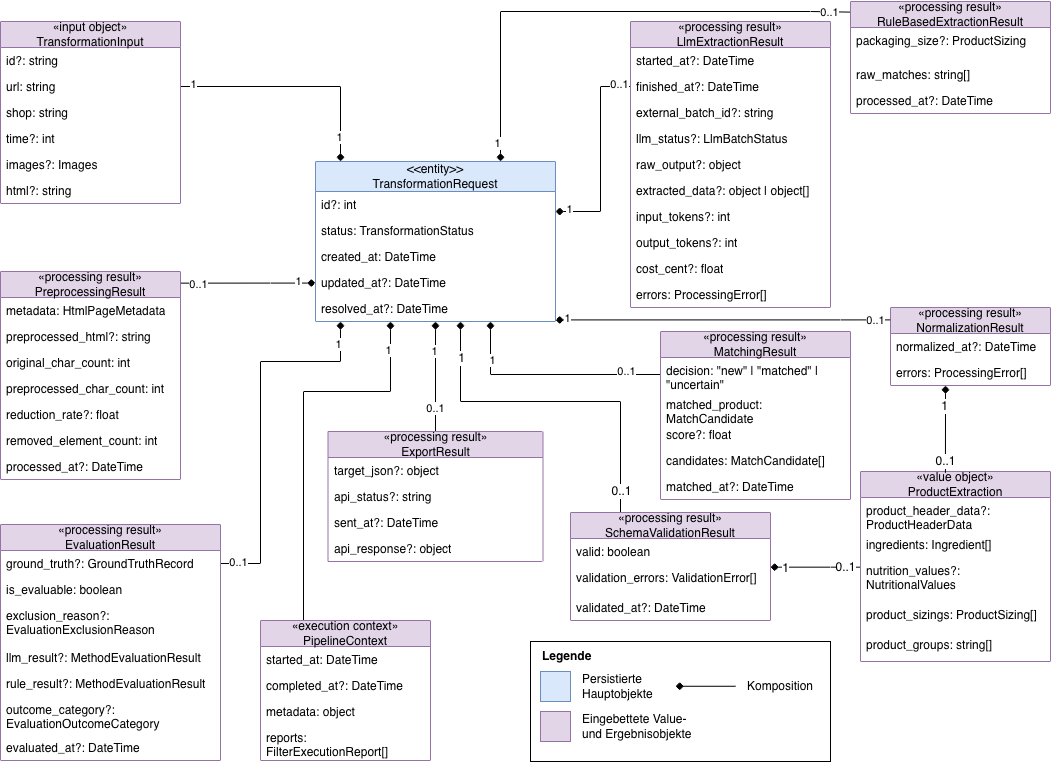
\includegraphics[width=\textwidth]{figures/DB_transformationRequest.png}
    \caption{Persistierter Verarbeitungskontext einer Transformationsanfrage}
    \label{fig:transformation-request-context}
\end{figure}

\paragraph{Persistierter Verarbeitungskontext:}

Abbildung~\ref{fig:transformation-request-context} löst den \textit{TransformationRequest} und seine eingebetteten Ergebnisobjekte weiter auf. Die ursprünglichen Quelldaten 
bleiben im \textit{TransformationInput} erhalten. Dadurch kann jedes erzeugte Ergebnis auf die ursprünglich übergebene Produktseite, den Shop, den HTML-Inhalt und die weiteren 
Eingabemetadaten zurückgeführt werden.

Das \textit{PreprocessingResult} speichert den durch das HTML-Cleanup erzeugten Produktkontext sowie Metadaten über den Umfang der Vorverarbeitung. Hierzu gehören insbesondere 
das vorverarbeitete HTML, die ursprüngliche und die verbleibende Zeichenanzahl sowie die Anzahl entfernter Elemente. Damit bleibt nachvollziehbar, auf welcher Eingabegrundlage 
die beiden Extraktionszweige gearbeitet haben.

Das Ergebnis der LLM-basierten Verarbeitung wird im \textit{LlmExtractionResult} gespeichert. Dieses enthält neben der Rohantwort und den daraus gelesenen Daten auch die 
externe Batchreferenz, den Bearbeitungsstatus des LLM-Dienstes, Zeitstempel, Tokenverbrauch, Kosteninformationen und mögliche Verarbeitungsfehler. Die Rohantwort bleibt 
erhalten, da die spätere Schema-Validierung nicht voraussetzen kann, dass jede LLM-Ausgabe bereits der erwarteten Struktur entspricht.

Parallel dazu wird das \textit{RuleBasedExtractionResult} als eigenständiger Bestandteil der Transformationsanfrage gespeichert. Es enthält das regelbasiert ermittelte 
\textit{ProductSizing} sowie die dafür berücksichtigten Rohkandidaten. Die getrennte Speicherung verhindert, dass das regelbasierte Resultat mit der umfassenderen 
LLM-basierten Produktextraktion vermischt wird. Beide Vorhersagen können dadurch innerhalb der Evaluation unabhängig voneinander derselben Ground Truth gegenübergestellt 
werden.

Die Schema-Validierung und die Normalisierung besitzen jeweils ein eigenes Ergebnisobjekt. Das \textit{SchemaValidationResult} enthält den validierten Stand der 
\textit{ProductExtraction} sowie festgestellte Strukturverletzungen. Das \textit{NormalizationResult} speichert den anschließend normalisierten Stand desselben fachlichen 
Datentyps und mögliche Normalisierungsfehler. Dadurch bleiben der validierte und der normalisierte Bearbeitungsstand voneinander unterscheidbar. Die \textit{ProductExtraction} 
fasst die strukturierte Produktextraktion zusammen, ohne im konzeptionellen Modell sämtliche verschachtelten Produktattribute aufzulösen.

Das \textit{MatchingResult} dokumentiert die Zuordnung zu einem lokal bekannten oder neu anzulegenden Produkt einschließlich der betrachteten Kandidaten und der getroffenen 
Entscheidung. Das \textit{EvaluationResult} speichert die auf Anfrageebene verwendete Ground Truth, die getrennten Resultate des LLM-basierten und des regelbasierten 
Ansatzes sowie die daraus abgeleitete Vergleichskategorie. Das \textit{ExportResult} hält schließlich den erzeugten Ziel-Payload und die technische Rückmeldung der Ziel-API 
fest. Die Evaluationsergebnisse sind nicht Bestandteil des an die Ziel-API übergebenen Produktobjekts.

Ergänzend können einer Transformationsanfrage mehrere \textit{PipelineContext}-Objekte zugeordnet werden. Sie enthalten Ausführungsberichte, Zeitinformationen und technische 
Metadaten der einzelnen Pipelineabschnitte. Während die Verarbeitungsergebnisse den fachlichen Zustand einer Produkttransformation abbilden, dokumentieren die 
Pipelinekontexte, unter welchen technischen Bedingungen diese Ergebnisse entstanden sind. Der \textit{TransformationRequest} fungiert damit als persistierter 
Verarbeitungskontext, anhand dessen eine Transformation fortgesetzt und nachträglich rekonstruiert werden kann.

\begin{figure}[H]
    \centering
    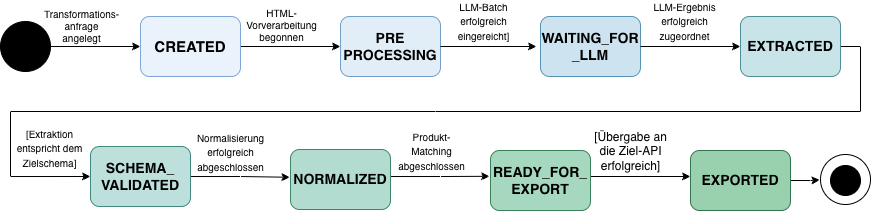
\includegraphics[width=\textwidth]{figures/Zustandsmodell_TR.png}
    \caption{Zustandsmodell einer Transformationsanfrage}
    \label{fig:transformation-request-state-model}
\end{figure}

\paragraph{Zustände einer Transformationsanfrage:}

Abbildung~\ref{fig:transformation-request-state-model} zeigt den regulären Erfolgsverlauf eines \textit{TransformationRequest}. Nach der Anlage befindet sich die Anfrage im 
Zustand \textit{CREATED}. Mit dem Beginn der HTML-Bereinigung wechselt sie in die Vorverarbeitungsphase \textit{PREPROCESSING}. Nach der erfolgreichen Einreichung des externen 
LLM-Batches wird \textit{WAITING\_FOR\_LLM} gesetzt. Dieser Zustand kennzeichnet die zeitliche Unterbrechung zwischen der lokalen Vorbereitung und der späteren Bereitstellung 
des LLM-Ergebnisses.

Nach dem erfolgreichen Abruf und der Zuordnung einer LLM-Antwort erreicht die Transformationsanfrage den Zustand \textit{EXTRACTED}. Darauf folgen die Zustände 
\textit{SCHEMA\_VALIDATED} und \textit{NORMALIZED}, sobald die extrahierten Produktdaten die strukturelle Prüfung beziehungsweise die Normalisierung erfolgreich durchlaufen 
haben. Nach Abschluss des Produkt-Matchings wird die Anfrage als \textit{READY\_FOR\_EXPORT} gekennzeichnet. Die Evaluation erzeugt keinen eigenen operativen Status und 
verändert diese Zustandsfolge nicht. Nach erfolgreicher Übergabe an die Ziel-API endet der reguläre Ablauf im Zustand \textit{EXPORTED}.

Zusätzlich kann eine Transformationsanfrage aus jedem noch nicht abgeschlossenen Verarbeitungszustand in den terminalen Zustand \textit{FAILED} wechseln. Dieser Zustand ist 
zugunsten der Übersicht nicht in Abbildung~\ref{fig:transformation-request-state-model} dargestellt. Ein Fehler einer einzelnen Anfrage wird auf dieser Ebene isoliert und 
verhindert nicht grundsätzlich die weitere Verarbeitung der übrigen Anfragen desselben Batches. Die konkreten Fehlerursachen und ihre Behandlung werden in Abschnitt~4.2.9 
beschrieben.

Der Zeitstempel \textit{resolved\_at} bezeichnet den Abschlusszeitpunkt des zuletzt ausgeführten Pipelineabschnitts. Er wird unabhängig davon aktualisiert, ob der jeweilige 
Abschnitt erfolgreich oder fehlerhaft beendet wurde. Der Zeitstempel kennzeichnet daher nicht ausschließlich den vollständigen Abschluss der gesamten Transformationsanfrage.

\begin{figure}[H]
    \centering
    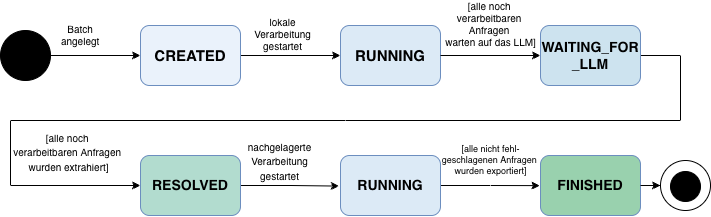
\includegraphics[width=\textwidth]{figures/Zustandsmodell_BR.png}
    \caption{Zustandsmodell eines Transformationsbatches}
    \label{fig:batch-request-state-model}
\end{figure}

\paragraph{Abgeleitete Batchzustände:}

Der Zustand eines \textit{BatchRequest} wird aus den Zuständen der enthaltenen Transformationsanfragen und aus batchweiten Verarbeitungsergebnissen abgeleitet. 
Abbildung~\ref{fig:batch-request-state-model} zeigt den regulären Verlauf. Nach der Anlage befindet sich der Batch zunächst in \textit{CREATED}. Sobald die lokale Verarbeitung 
beginnt, wechselt er in \textit{RUNNING}. Warten alle noch verarbeitbaren Anfragen auf die externe LLM-Verarbeitung, erhält der Batch den Zustand \textit{WAITING\_FOR\_LLM}.

Sind die LLM-Ergebnisse für alle noch verarbeitbaren Anfragen zugeordnet, wird der Zustand \textit{RESOLVED} erreicht. Dieser Zustand kennzeichnet den Abschluss der externen 
Extraktionsphase, nicht den Abschluss des gesamten Transformationslaufs. Mit dem separaten Start der nachgelagerten Verarbeitung wechselt der Batch erneut in \textit{RUNNING}. 
Sobald alle nicht fehlgeschlagenen Transformationsanfragen erfolgreich an die Ziel-API übergeben wurden, endet der Batch im Zustand \textit{FINISHED}.

Einzelne fehlgeschlagene Transformationsanfragen führen nicht zum Batchstatus \textit{FAILED}. Ein Batch kann deshalb auch dann \textit{WAITING\_FOR\_LLM}, \textit{RESOLVED} 
oder \textit{FINISHED} erreichen, wenn einzelne Requests bereits als fehlgeschlagen markiert wurden. Der Umfang partieller Fehler bleibt über den \textit{failed\_count} der 
Batchzusammenfassung sichtbar. Der Batchstatus \textit{FAILED} wird nur gesetzt, wenn keine sinnvolle Fortsetzung des gesamten Batches mehr möglich ist. Dies ist insbesondere 
der Fall, wenn alle Transformationsanfragen fehlgeschlagen sind oder ein nicht behebbarer batchweiter Fehler sämtliche noch offenen Anfragen betrifft.

\paragraph{Persistenzstrategie:}

Die lokalen Arbeitsobjekte werden schrittweise persistiert. Nach jedem Pipelineabschnitt werden der aktuelle Zustand, die neu entstandenen Ergebnisobjekte und die zugehörigen 
Ausführungsinformationen gespeichert. Dadurch kann die Verarbeitung nach der zeitlich getrennten LLM-Ausführung fortgesetzt werden, ohne die bereits abgeschlossenen Schritte 
erneut ausführen zu müssen. Gleichzeitig bleiben Rohdaten, Zwischenergebnisse, externe Antworten, Matching-Entscheidungen, Bewertungen und Exportresultate einer konkreten 
Transformationsanfrage zugeordnet.

Die lokale MongoDB speichert die Batches, Transformationsanfragen und Produktdaten als Arbeits-, Transformations- und Evaluationsdaten. Ergebnis- und Kontextobjekte werden 
als Bestandteile der jeweils übergeordneten Arbeitsobjekte verwaltet. Die Ground Truth bleibt als getrennte Referenzdatenbasis erhalten. Die lokale Persistenz ersetzt nicht 
die produktive Datenhaltung, Transformierte Produktdaten werden ausschließlich über die Ziel-API an das nachgelagerte System übergeben. Dateibasierte Evaluationsberichte 
sind aus den persistenten Einzel- und Batchbewertungen abgeleitete Artefakte und bilden keine zusätzliche führende Datenquelle.

Das Daten-, Zustands- und Persistenzkonzept schafft damit die Voraussetzung für die mehrphasige Verarbeitung, die Isolation einzelner Fehler sowie die spätere wissenschaftliche 
Auswertung. Der folgende Abschnitt betrachtet die Schnittstellen, über die die dargestellten Arbeitsobjekte und Ergebnisse mit Eingabeadaptern, externen Diensten und dem 
Zielsystem ausgetauscht werden.

\subsubsection{Schnittstellen- und Integrationskonzept}

Die Systemgrenzen des CrawlDataTransformer werden durch fachlich definierte Ports gekapselt. Technische Adapter übersetzen externe Eingabe-, Speicher- und Ausgabeformate in die 
internen Modelle beziehungsweise aus diesen heraus. Dadurch bleibt die Transformationslogik von konkreten Übertragungsprotokollen, Datenbankstrukturen und anbieterspezifischen 
Schnittstellen getrennt. Tabelle~\ref{tab:interface-overview} fasst die wesentlichen Integrationen zusammen.

\begin{table}[H]
    \centering
    \footnotesize
    \renewcommand{\arraystretch}{1.15}
    \begin{tabular}{
        |p{0.19\textwidth}
        |p{0.25\textwidth}
        |p{0.43\textwidth}|
    }
        \hline
        \textbf{Schnittstelle} &
        \textbf{Integration} &
        \textbf{Funktion und Besonderheit} \\
        \hline

        Eingabe &
        REST und CLI &
        Überführung unterschiedlicher Eingabeformate in gemeinsame interne Modelle und Aufruf derselben Anwendungsfälle \\
        \hline

        LLM-Extraktion &
        Gemini Batch API &
        Getrennte Einreichung und Ergebnisabfrage über eine persistierte externe Batchreferenz \\
        \hline

        Produkt-Matching &
        Gemini API &
        Synchroner Aufruf zur optionalen semantischen Unterstützung der Matching-Entscheidung \\
        \hline

        Persistenz &
        Lokale MongoDB &
        Speicherung von Arbeits-, Zustands-, Produkt- und Evaluationsdaten über Repository-Schnittstellen \\
        \hline

        Produktexport &
        Ziel-API &
        Abbildung auf das externe Zielmodell und ausschließlich schnittstellenbasierte produktive Übergabe \\
        \hline

        Bewertungsexport &
        Dateisystem &
        Vom Produktexport getrennte Bereitstellung der Evaluationsdaten \\
        \hline
    \end{tabular}
    \caption{Schnittstellen und Integrationen des CrawlDataTransformer}
    \label{tab:interface-overview}
\end{table}

Auf der Eingabeseite greifen die REST-Schnittstelle und die Kommandozeilenschnittstelle über denselben Eingangsport auf den Anwendungskern zu. Beide Adapter überführen ihre 
jeweiligen Eingabestrukturen in gemeinsame Modelle für Transformationsdaten, Batchherkunft und Konfiguration. Der verwendete Eingabekanal verändert daher weder die 
fachliche Verarbeitung noch die nachfolgenden Integrationen.

Die LLM-basierte Extraktion berücksichtigt die zeitliche Trennung zwischen Einreichung und Ergebnisbereitstellung. Getrennte Ausgangsports kapseln die Übermittlung 
eines Batches sowie die spätere Statusprüfung und Ergebnisabfrage. Die dabei erhaltene externe Batchreferenz wird persistiert und ermöglicht die Zuordnung der später 
bereitgestellten Antworten zu den ursprünglichen Transformationsanfragen. Anbieterbezogene Status- und Antwortformate werden durch die Adapter in interne Ergebnisobjekte 
überführt. Davon getrennt verwendet das Produkt-Matching einen synchronen Port, da eine mögliche semantische Unterstützung unmittelbar innerhalb der nachgelagerten 
Verarbeitung benötigt wird.

Für die lokale Datenhaltung definiert der Anwendungskern Repository-Schnittstellen für Batches, Transformationsanfragen, Produkte und Referenzdaten. Die konkrete 
Abbildung auf MongoDB-Dokumente verbleibt in den Persistenzadaptern. Dadurch werden datenbankspezifische Strukturen nicht Bestandteil der fachlichen Filter.

Auch die ausgehenden Integrationen sind voneinander getrennt. Vor dem Produktexport wird die interne Produktdarstellung auf das erwartete Zielmodell abgebildet und 
anschließend über den Exportport an die Ziel-API übertragen. Die Ziel-API übernimmt die produktive Validierung und Speicherung. Ein direkter Schreibzugriff auf die 
produktive Datenbank erfolgt nicht. Der Bewertungsexport stellt dagegen ausschließlich Evaluationsdaten dateibasiert bereit und verändert das exportierte Produktobjekt 
nicht. Die Behandlung von Kommunikations- und Integrationsfehlern wird in Abschnitt~4.2.9 beschrieben.

\subsubsection{Evaluations- und Nachvollziehbarkeitskonzept}

Die Evaluation ist als optionaler und vom produktiven Export getrennter Verarbeitungsschritt konzipiert. Sie vergleicht die Ergebnisse der LLM-basierten und der 
regelbasierten Extraktion für das Referenzdatenfeld \textit{ProductSizing}, beeinflusst jedoch weder die Exportfreigabe noch den operativen Status einer erfolgreich 
transformierten Anfrage. Produktdaten können daher auch dann verarbeitet werden, wenn keine auswertbare Ground Truth vorliegt.

Die Bewertung erfolgt zunächst auf Ebene eines \textit{TransformationRequest}. Die Ground Truth wird über die Kennung der ursprünglichen Eingabe zugeordnet. Als auswertbar 
gelten sowohl annotierte Verpackungsgrößen als auch bestätigte Fälle ohne vorhandene Verpackungsgröße. Unsichere, übersprungene, fehlende oder nicht eindeutig zuordenbare 
Referenzdaten werden von den Qualitätsmetriken ausgeschlossen und mit ihrem Ausschlussgrund dokumentiert.

Verglichen werden die normalisierten Werte und Einheiten der Extraktionsergebnisse. Eine Übereinstimmung liegt vor, wenn sämtliche zu vergleichenden 
\textit{ProductSizing}-Werte der Ground Truth beziehungsweise der regelbasierten Extraktion in der Liste der LLM-basierten Ergebnisse enthalten sind. Zusätzliche 
LLM-Ergebnisse verhindern die Übereinstimmung nicht, werden jedoch als mögliche Überextraktion gesondert berücksichtigt. Die Einzelbewertungen erfassen unter anderem 
Übereinstimmungen und Abweichungen bei Wert, Einheit und Dimension sowie fehlende oder unbelegte Vorhersagen. Anschließend werden die Ergebnisse auf Batch-Ebene zu 
technischen und methodenspezifischen Kennzahlen zusammengeführt. Hierzu zählen beispielsweise Schema- und Normalisierungserfolg, Precision, Recall, F1-Score, 
Übereinstimmungsraten, Fehlerverteilungen, Tokenverbrauch, Kosten und lokale Verarbeitungsdauer. Die verbindlichen Definitionen und Berechnungsgrundlagen werden in 
Abschnitt~6.1.2 festgelegt.

Die Nachvollziehbarkeit wird durch die gemeinsame Persistierung der ursprünglichen Eingabe, des vorverarbeiteten HTML, der Extraktions- und Normalisierungsergebnisse, der 
regelbasierten Vorhersage, der Ground Truth sowie der Einzelbewertung unterstützt. Pipelinekontexte ergänzen diese Daten um Status, Ausführungsdauer und Fehlermeldungen 
der Verarbeitungsschritte. Die Einzel- und Batchbewertungen bilden die maßgebliche Datenbasis. Der dateibasierte Bewertungsexport stellt daraus abgeleitete Artefakte für 
die wissenschaftliche Auswertung bereit.

\subsubsection{Status- und Fehlerbehandlungskonzept}

Die Fehlerbehandlung unterscheidet zwischen requestlokalen und batchweiten Fehlern. Datenbezogene Probleme wie nicht parsebare LLM-Antworten, Schemaabweichungen, fehlende 
Zwischenergebnisse oder abgelehnte Exporte betreffen zunächst nur den jeweiligen \textit{TransformationRequest}. Technische Fehler können innerhalb eines Verarbeitungsschritts, 
bei der Persistenz oder bei der Kommunikation mit externen Diensten auftreten. Sie werden möglichst nahe an der verursachenden Verarbeitungsstufe erfasst.

Jeder Filter verarbeitet nur Anfragen in einem dafür vorgesehenen Eingangszustand. Erwartete Abweichungen werden soweit möglich in den jeweiligen Ergebnisobjekten dokumentiert, 
beispielsweise durch Validierungsfehler mit dem betroffenen Datenpfad oder Verarbeitungsfehler mit Fehlercode und Beschreibung. Kann eine Anfrage nicht sinnvoll fortgesetzt 
werden, wechselt sie in den terminalen Zustand \textit{FAILED}. Die übrigen Anfragen desselben Batches können weiterhin verarbeitet werden.

Unerwartete Ausnahmen werden durch die Pipelineausführung abgefangen und mit dem betroffenen Filter, seiner Ausführungsdauer und der Fehlermeldung im Pipelinekontext 
gespeichert. Der technische Ausführungsstatus eines Filters ist dabei vom fachlichen Ergebnis zu unterscheiden: Ein Filter kann ohne Ausnahme ausgeführt werden und dennoch 
einen fachlichen Fehler feststellen. Eine allgemeine automatische Wiederholung fehlgeschlagener Schritte ist im Prototyp nicht vorgesehen.

Der Batchstatus wird aus den Zuständen der noch verarbeitbaren Anfragen abgeleitet. Einzelne fehlgeschlagene Requests werden über ihre Zustände und den \textit{failed\_count} 
sichtbar, führen jedoch nicht zum Abbruch des Batches. Der Batchstatus \textit{FAILED} wird nur gesetzt, wenn keine sinnvolle Fortsetzung möglich ist, etwa weil alle Anfragen 
fehlgeschlagen sind oder ein endgültiger Fehler des externen LLM-Batches sämtliche offenen Anfragen betrifft. Ein Batch mit erfolgreich exportierten und fehlgeschlagenen 
Anfragen endet dagegen als \textit{FINISHED}.